\documentclass{article} % For LaTeX2e
\usepackage[final]{../colm2025_conference}

\usepackage{microtype}
\usepackage{hyperref}
\usepackage{url}
\usepackage{amsthm}
\usepackage{amsmath}
\usepackage{amssymb}
\usepackage{pifont}% http://ctan.org/pkg/pifont
\usepackage{booktabs}
\usepackage{soul}
\usepackage{cancel}
\usepackage{algorithm}
\usepackage{algpseudocode}
\usepackage{graphicx}
\usepackage{subfig}
\usepackage{tablefootnote}
\theoremstyle{definition}
\newtheorem{theorem}{Theorem}[section]
% \newtheorem{proof}{Proof}[section]

\usepackage{lineno}
\newcommand{\cmark}{\ding{51}}%
\newcommand{\xmark}{\ding{55}}%

\definecolor{darkblue}{rgb}{0, 0, 0.5}
\hypersetup{colorlinks=true, citecolor=darkblue, linkcolor=darkblue, urlcolor=darkblue}


\title{Week 8: Pre-Training with nanoGPT}

\author{\textbf{BEH} Chuen Yang}

\newcommand{\fix}{\marginpar{FIX}}
\newcommand{\new}{\marginpar{NEW}}

\begin{document}

\ifcolmsubmission
\linenumbers
\fi

\maketitle

\begin{abstract}
    This report explores language model pre-training with the help
    of nanoGPT (\cite{nanoGPT}), a simple and efficient implementation of the GPT architecture
    in PyTorch. We use a small dataset (\cite{tinyss}) of $\sim$1M tokens (Shakespeare's works)
    to train a small-scale GPT model, and qualitatively evaluate its
    text generation capabilities.
\end{abstract}

\section{Motivation}
Pre-training is the most essential step in creating a language model.
It is from this step that the model gains a baseline, causal understanding of language,
in which words depend only on the words that precede them.

While training deep neural networks to just "predict next token" is a very straightforward process,
pre-training's apparent simplicity belies the difficulty of getting language models to go from
outputting garbage to "understanding" text, much less the challenges involved in translating that
"understanding" into fluent text generation.

Hence, it is essential to have hands-on experience with pre-training in order to appreciate
some of these challenges in greater detail. 

\section{nanoGPT}
In order to gain this experience quickly, we will use nanoGPT (\cite{nanoGPT}), a simple and efficient 
implementation of the GPT architecture in PyTorch.

Not only is the code concise and relatively easy to understand, it also
comes with a number of features that make it suitable for experimentation:
\begin{itemize}
    \item Configuration files for different datasets and model architectures, 
        further customisable via command line arguments.
    \item Automatic model compilation and mixed precision support
        for training models on less powerful computers.
    \item One-file training and evaluation scripts that encapsulate the relevant logic.
    \item WandB (\cite{wandb}) integration for convenient logging.
\end{itemize}

Obviously, nanoGPT does not come with many of the most advanced features
that are in today's state-of-the-art language models. However,
it is just as good for witnessing the pre-training process in action,
as the way the pre-training works (once the data is prepared) is very similar
to how it is done in larger models.

\subsection{Training Code Analysis}
While the repository comes with a number of files and scripts,
we will focus only on the essential ones for this week's report.

The following table contains brief descriptions of said essential files,
and we will elaborate on the high-level components they implement 
in the following subsections.

\begin{table}
    \centering
    \begin{tabular}{|p{0.3\textwidth}|p{0.7\textwidth}|}
        \hline
        \textbf{File Path} & \textbf{Description} \\
        \hline
        data/shakespeare\_char/ \newline prepare.py 
        & Script to prepare the Tiny Shakespeare dataset (\cite{tinyss}) for training.
        \\ \hline
        configurator.py & 
        Assists in loading configuration files and command line arguments.
        \\ \hline
        config/ \newline train\_shakespeare\_char.py 
        & Sample configuration file for the Shakespeare dataset.
        \\ \hline
        config/ \newline train\_shakespeare \newline \_char\_modified.py 
        & Modified configuration file for the Shakespeare dataset. \newline
        Changes were restricted to batch size and model specifications.
        \\ \hline
        model.py & Implementation of the GPT model.
        \\ \hline
        train.py & Main training script that handles data loading, training loop, and logging.
        \\ \hline
        evaluate.py & Evaluation script that generates text from the trained model.
        \\ \hline
    \end{tabular}
    \caption{Essential files in the nanoGPT (\cite{nanoGPT}) repository}
    \label{tab:nanogpt_files}
\end{table}

\subsection{Dataset \& Data Preparation}

Corresponding File: \texttt{data/shakespeare\_char/prepare.py}

The dataset we will focus on for this report is the Tiny Shakespeare dataset (\cite{tinyss}),
which purportedly contains the complete works of William Shakespeare in a single text file (\cite{tinyss2}).
\footnote{
    Despite claiming to contain all of Shakespeare's works, the dataset seems to be missing
    some works, most notably, \textit{Julius Caesar}.
}

To obtain tokens for training, 
\begin{itemize}
    \item \texttt{data/shakespeare\_char/prepare.py} downloads this dataset,
    \item records metadata about the dataset (like the vocabulary, total token counts, etc.),
    \item splits the data (90\% train, 10\% validation) into training and validation sets,
    \item tokenizes each text block on a character level,
    \item and saves both the (tokenized) training and validation corpuses to disk.
\end{itemize}

This creates a training dataset with $\sim$ 1M tokens (since there are $\sim$ 1.1M characters in the text),
which is vanishingly small relative to traditional pre-training corpuses (\cite{beh-2025}).
However, the small size also allows us to pre-train a small model in a reasonable amount of time,
and to quickly iterate on the training process.

During pre-training, only the train set is used, and the validation set is used
to provide diagnostic information about the model's performance on unseen data.

\subsection{Model Architecture}
Corresponding File: \texttt{model.py}

\begin{figure}[h]
    \centering
    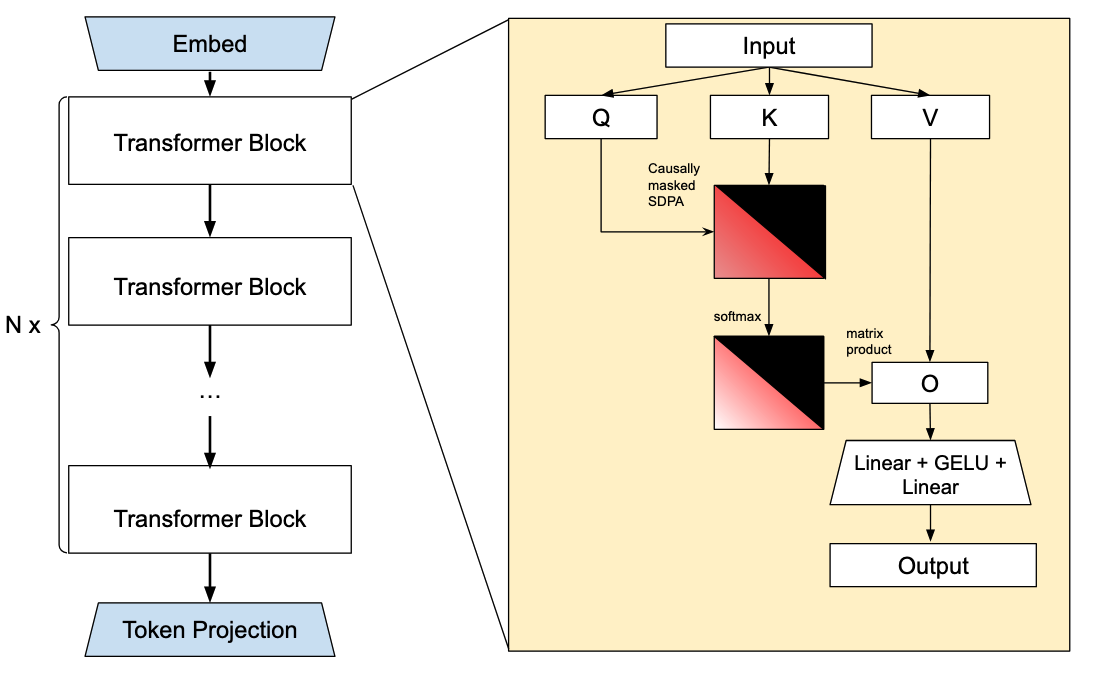
\includegraphics[width=0.8\textwidth]{images/gpt_arch.png}
    \caption{nanoGPT (\cite{nanoGPT}) model architecture}
    \label{fig:nanogpt_architecture}
\end{figure}

Since GPT is its namesake, it should be unsurprising that nanoGPT closely follows 
the GPT architecture (\cite{radford-et-al-2019}), which is itself 
a relatively simple decoder-only transformer (\cite{vaswani-et-al-2017}).
Figure \ref{fig:nanogpt_architecture} shows the architecture of the model at a glance.

There are, however, two notable departures from the GPT architecture:
\begin{itemize}
    \item The activation function used in the model is Gaussian Error Linear Unit (GELU) (\cite{gelu}),
rather than the more common ReLU or LeakyReLU (\cite{xu-et-al-2015, relu}).
\end{itemize} 


\subsection{Training Loop}
Corresponding File: \texttt{train.py}

As mentioned in \cite{beh-2025}, language model pre-training
is typically formulated as a self-supervised, next-token prediction task,
and nanoGPT is no exception. Algorithm \ref{alg:nanogpt_training_loop} shows 
provides a sketch of the training loop used in nanoGPT.

% In sum, the loop works as follows:
% \begin{itemize}
%     \item From the training tokens, extract contiguous blocks of tokens
%         with the same length as the model's context window.
%     \item For each block, create a corresponding target block
%         where the $n$-th token in the target block generally corresponds 
%         to the $(n+1)$-th token in the input block. 
%         In particular, the last token in the target block corresponds 
%         to the first token after the input block.
%     \item Feed the input block to the model to extract next-token logits
%         for each position in the block.
%     \item Using the target block as ground-truth, compute the average cross-entropy loss
%         between the model's logits and the target tokens across the sequence and batch dimensions
%     \item Backpropagate the loss and update the model's parameters.
% \end{itemize}

\begin{algorithm}[H]
\caption{nanoGPT Training Loop (Next-Token Prediction)}
\begin{algorithmic}[1]
\Require Training corpus $\mathcal{T} = [t_1, t_2, \ldots, t_N]$, context window size $C$, batch size $B$, Model parameters $\theta$
% \algorithmicreturn~ $\theta$ after training
\While{not converged}
    \State Sample $B$ indices $\{s_1, \ldots, s_B\}$ uniformly at random such that $\forall b (s_b + C \leq N)$
    \For{$b = 1$ to $B$}
        \State $\mathbf{x}^{(b)} \gets [t_{s_b}, t_{s_b+1}, \ldots, t_{s_b+C-1}]$ \Comment{Input block}
        \State $\mathbf{y}^{(b)} \gets [t_{s_b+1}, t_{s_b+2}, \ldots, t_{s_b+C}]$ \Comment{Target block (shifted by 1)}
    \EndFor
    \State Stack $\{\mathbf{x}^{(b)}\}_{b=1}^B$ into input batch $\mathbf{X} \in \mathbb{N}^{B \times C}$
    \State Stack $\{\mathbf{y}^{(b)}\}_{b=1}^B$ into target batch $\mathbf{Y} \in \mathbb{N}^{B \times C}$
    \State Compute logits $\mathbf{L} = \mathrm{Model}(\mathbf{X}) \in \mathbb{R}^{B \times C \times V}$, where $V$ is vocab size
    \State Compute loss $\mathcal{L} = \mathrm{CrossEntropy}(\mathbf{L}, \mathbf{Y})$ (averaged over batch and sequence)
    \State Backpropagate $\mathcal{L}$ and update $\theta$
\EndWhile
\end{algorithmic}
\end{algorithm}

\subsection{Evaluation Loop}
Corresponding File: \texttt{evaluate.py}

nanoGPT provides autoregressive evaluation of trained models, as is usual
for language models. Starting with a user-provided prompt,

\begin{itemize}
    \item the script generates logits by performing a forward pass through the model
    \item samples the next token from the \textbf{LAST} token's logits,
    \item appends the sampled token to the prompt,
    \item and repeats the process until the desired number of tokens is generated.
\end{itemize}

Since only full blocks of tokens are ever used during training,
one would not be faulted for suspecting that the model may
not properly learn to generate text in an autoregressive manner,
especially if the prompt itself is not a full block of tokens.

However, this is not the case. Further explanation can be found
in Appendix \ref{sec:appendix_autoregressive}.

\section{Training Runs}
\subsection{Training Configuration}
Table \ref{tab:training-hyperparameters} summarises the salient hyperparameters used for training.
If any more details are desired, they can be found in \texttt{config/train\_shakespeare\_char\_modified.py}.

% TODO: CHECK THE VALUES AGAINST THE CONFIG FILE LATER!!!
\begin{table}
    \centering
    \begin{tabular}{|p{0.3\textwidth}|p{0.35\textwidth}|}
        \hline
        \textbf{Hyperparameter} & \textbf{Value} \\ \hline
        Context Window & 512 tokens \\ \hline
        Batch Size & 32 samples \\ \hline
        \# Layers & 12 \\ \hline
        \# Attention Heads & 8 \\ \hline
        Embedding Dimension & 256 \\ \hline
        Dropout Rate & 0.2 \\ \hline
        Learning Rate & 1e-3 \\ \hline
        Weight Decay & 1e-1 \\ \hline
        Training Steps & 5000 \\ \hline
        Optimizer & AdamW, $\beta_1 = 0.9, \beta_2 = 0.99$ (\cite{adamw})\\ \hline
        Batching Seed & 1337 \\ \hline
    \end{tabular}
    \caption{Training hyperparameters for the modified Shakespeare model}
    \label{tab:training-hyperparameters}
\end{table}

Training was done on 1x NVIDIA RTX A2000 GPU with 8GB of VRAM 
with BF16 automatic mixed precision. The full run took approximately 15 minutes.

\subsection{Loss Curves}

Figure \ref{fig:loss_curves} shows the training and validation loss curves
for the training run. 

\begin{figure}[h]
    \centering
    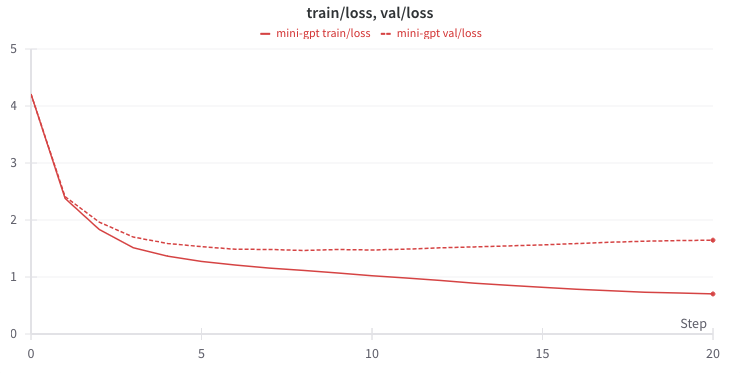
\includegraphics[width=0.8\textwidth, height=0.25\textheight]{images/loss_curves.png}
    \caption{Training and validation loss curves for the modified Shakespeare model.  Note that the losses were only recorded every 250 steps.}
    \label{fig:loss_curves}
\end{figure}

\section{Evaluations \& Discussion}

For evaluations, we allowed the model to autoregressively continue a given prompt
for 200 tokens, and repeated this process 10 times for each prompt.

As with the previous section, the salient hyperparameters can be found in 
Table \ref{tab:eval-hyperparameters}. \footnote{
    Technically, Karpathy leverages top-k sampling in his script (\cite{nanoGPT}).
    However, a manual inspection of the dataset reveals there are only 65 unique characters,
    much less than his top-k of 200. Hence the top-k is effectively a no-op.
}

\begin{table}
    \centering
    \begin{tabular}{|p{0.275\textwidth}|p{0.35\textwidth}|}
        \hline
        \textbf{Hyperparameter} & \textbf{Value} \\ \hline
        Sampling Temperature & 0.6 \\ \hline
        \# Samples per Prompt & 10 \\ \hline
        Sampling Seed & 1337 \\ \hline
        Prompt 1 & "Beware the ides of March." \tablefootnote{
            The prompt is derived from the famous line in \textit{Julius Caesar} (Act 1, Scene 2).
            Since the line was not found in the input corpus, 
            it qualifies as out-of-distribution (OOD) data.
        }\\ \hline
        Prompt 2 & "Who are you?" \tablefootnote{
            Another OOD prompt to maintain parity with \cite{beh-2025-b}.
        }\\ \hline
        Prompt 3 & "What is the range of output of tanh?" \tablefootnote{
            Another OOD prompt to maintain parity with \cite{beh-2025-b}.
        } \\ \hline
    \end{tabular}
    \caption{Evaluation hyperparameters for the modified Shakespeare model.}
    \label{tab:eval-hyperparameters}
\end{table}

We then compared the generated text against texts 
from the small Qwen models from last week's report (\cite{beh-2025-b}),
using the same sampling temperature.

For the sake of brevity, we will not include the full text generation results here
(although the texts generated by our pre-trained model can be found in 
\texttt{out-shakespeare-char}, and the Qwen models' outputs can be found from \cite{beh-2025-b}).
Instead, we will summarise the results in the following subsections,
referring to the model we pre-trained as "nanoGPT".

\subsection{Text Generation Format}
As a result of its training set, nanoGPT generates text similar in format
to Shakespeare's works (\texttt{$<$NAME$>$:$\backslash$ n$<$LINE 1$>\backslash$ n$<$LINE 2$>\backslash$ n...$\backslash$ n$\backslash$ n}),
where each line starts with a capital letter, without fail.

However, any similarities appear to be textual, and indeed quite superficial in nature,
as the model \textit{frequently repeats the same interlocutors' names} in the generated text,
and notably \textit{does not understand the iambic pentameter} structure in which Shakespeare's 
works are written. Take for example, this contiguous piece of dialogue generated by nanoGPT:
\begin{quote}
DUKE OF YORK:

The letters will the sun sue of England's death. (11 syllables)

DUKE OF YORK:

Why looks thou comest to the Duke of Norfolk? (11 syllables)
\end{quote}


By contrast, the Qwen models were able to generate text in a wider variety of formats
and styles, including multiple choice, and so on. If instruct-tuned, Qwen models
are also able to generate text in a more conversational style.

\subsection{Text Generation Quality}
Surprisingly for a model that is tokenized on a character level,
nanoGPT is able to \textit{generate whole words}, with \textit{little to no character-level errors}.

Beyond that, nanoGPT's text is \textit{completely nonsensical} at a phrase and sentence level.
nanoGPT also appears to constantly \textit{remix and regurgitate} different variations
of quasi-Shakespearean dialogue, using phrases like "I prithee", "sir" and "my lord" frequently,
but never in a coherent manner. For example, it might generate sentences like:
\begin{quote}
    I do not, sir, my lord. 
\end{quote}

All these indicate that nanoGPT does not understand the meaning of the words it generates,
and is simply regurgitating phrases it has seen in the training set.

By contrast, the Qwen models mostly generated cogent and natural sentences,
and were on occasion even able to answer questions in a conversational manner (\cite{beh-2025-b}).

\subsection{Discussion}
When analyzing the results side by side with the loss curves,
it is quite clear that nanoGPT has somewhat learnt the structure of Shakespeare's works,
as evidenced by the steady decrease in training and validation loss
over the course of training. Nevertheless, it quite obviously and dismally fails 
to generate text reminiscent of natural language as it is spoken/written today.

Considering that nanoGPT is a relatively good implementation of the GPT architecture,
and that manual inspections have yet to identify any glaring bugs in the model architecture
and training loop, it is \textbf{likely that the model's failure to generate coherent text
stems from}: 
\begin{itemize}
    \item the small size of the training set
    \item the restricted domain of the training set (i.e. most of Shakespeare's works)
    \item the small size of the model itself
\end{itemize}

\section{Conclusion}
In this report, we have explored the pre-training process of a small language model
using nanoGPT (\cite{nanoGPT}). Through this small yet well-made library, 
we have seen how the pre-training process works,
run a pre-training run on a small dataset,
and qualitatively evaluated the model's text generation capabilities.
In short, we have effectively witnessed the full pre-training pipeline in action.

While the model was able to learn some of the structure of Shakespeare's works,
it ultimately failed to generate coherent text despite an apparently robust implementation
and training process.
This serves as a reminder of the challenges involved in pre-training language models,
and the importance of large datasets and model sizes in achieving good performance.

\bibliographystyle{../colm2025_conference}
\bibliography{wk8}

\appendix

\section{Appendix: Why Full Block Training Lends Itself Well to Autoregressive Generation}
\label{sec:appendix_autoregressive}

Examining the source code, we find that the \texttt{CasualSelfAttention}
module is designed to project embedding tokens in parallel (line 56).

Moreover, due to the theorem below, the casual self-attention matrix 
is invariant to the suffix of the input sequence:

\begin{theorem}[Causal Attention Prefix Invariance]
Let $\mathbf{X} = (\mathbf{x}_1 | \mathbf{x}_2 | \ldots | \mathbf{x}_n) \in \mathbb{R}^{d \times n}$ be a sequence of token embeddings, 
and let $\mathbf{W}_Q, \mathbf{W}_K \in \mathbb{R}^{d_{att} \times d}$ be the query and key projection matrices for a self-attention head.

Define the masked attention scores as 
\begin{equation}
\mathbf{B}(\mathbf{X})_{ij} = \frac{\exp(\mathbf{A}(\mathbf{X})_{ij})}{\sum_{k=1}^{n} \exp(\mathbf{A}(\mathbf{X})_{ik})}
\end{equation}

where $\mathbf{A}(\mathbf{X})_{ij} = 
\begin{cases}
    \frac{(\mathbf{W}_Q \mathbf{x}_i)^T (\mathbf{W}_K \mathbf{x}_j)}{\sqrt{d_{att}}} & \text{if } j \leq i \\
    -\infty & \text{if } j > i
\end{cases}$

Then for any prefix length $m < n$, $\mathbf{B}(\mathbf{X})_{1:m,1:m} = \mathbf{B}(\mathbf{X}_{1:m})$.
\end{theorem}

\begin{proof}
    % Notice that 
    % $$\begin{array}{rl}
    %    \mathbf{A}(\mathbf{X}_{1:m})_{ij} &= 
    %     \begin{cases}
    %         \frac{(\mathbf{W}_Q \mathbf{x}_i)^T (\mathbf{W}_K \mathbf{x}_j)}{\sqrt{d_{att}}} & \text{if } 1 \leq j \leq i \leq m \\
    %         -\infty & \text{otherwise}
    %     \end{cases} \\
    %     & = 
    %     \begin{cases}
    %         \mathbf{A}(\mathbf{X})_{ij} & \text{if } 1 \leq j \leq i \leq m \\
    %         -\infty & \text{otherwise}
    %     \end{cases} \\
    %     & = \mathbf{A}(\mathbf{X})_{1:m, 1:m}
    % \end{array}$$


    Since $i \leq m$, all positions $k \leq i$ are within the prefix $\mathbf{X}_{1:m}$. Therefore:
    \begin{equation}
        \mathbf{A}(\mathbf{X})_{ij} = \mathbf{A}(\mathbf{X}_{1:m})_{ij} \quad \text{for all } j \leq i \leq m
    \end{equation}

    Since we conduct softmax over the last dimension we only care about the case when $j > m$ but $i \leq m$.
    Here, naturally $j > i$.
    Hence, we have
    % $$\begin{array}{rl}
    %     \mathbf{B}(\mathbf{X})_{1:m, 1:m} &= softmax(\mathbf{A}(\mathbf{X})_{1:m, 1:m}, dim = -1) \\
    %     & = softmax(\mathbf{A}(\mathbf{X}_{1:m}), dim = -1) \\
    %     & = \left( \begin{array}{c|c}
    %         \mathbf{B}(\mathbf{X}_{1:m}) & \mathbf{0} \\ \hline
    %         \mathbf{0} & \mathbf{0}
    %     \end{array}\right)_{1:m, 1:m} \\
    %     & = \mathbf{B}(\mathbf{X}_{1:m})
    % \end{array}$$

    \begin{align*}
        \mathbf{B}(\mathbf{X})_{ij} &= \frac{\exp(\mathbf{A}(\mathbf{X})_{ij})}{\sum_{k=1}^{n} \exp(\mathbf{A}(\mathbf{X})_{ik})} \\
        &= \frac{\exp(\mathbf{A}(\mathbf{X}_{1:m})_{ij})}{\sum_{k=1}^{m} \exp(\mathbf{A}(\mathbf{X}_{1:m})_{ik})} \\
        &= \mathbf{B}(\mathbf{X}_{1:m})_{ij}
    \end{align*}

\end{proof}

As such, it does not matter how much of the model's context window is used
to generate the next token. If I had any $m < n$ for a sequence length $n$, 
the top left $m \times m$ block of the causal attention matrix would be the same 
as the causal attention matrix calculated using only the first $m$ tokens
of the sequence.

To reiterate, nanoGPT will be able to autoregressively generate text
just fine, even if the prompt is not a full block of tokens.

\end{document}